\documentclass[12pt, a4paper]{article}

% ==========================================
% 1. KHAI BÁO GÓI THƯ VIỆN (PACKAGES)
% ==========================================
% Bảng mã & Font chữ
\usepackage[utf8]{inputenc}
\usepackage[T5]{fontenc}

% Toán học
\usepackage{amsmath, amssymb}

% Căn lề & Bố cục trang
\usepackage[top=2.2cm, bottom=1.5cm, left=1cm, right=1cm, headheight=15pt]{geometry}
\usepackage{fancyhdr}
\usepackage{needspace}
\usepackage{tkz-tab}

% Đồ họa & Màu sắc
\usepackage{xcolor}
\usepackage{graphicx} 
\usepackage{tikz}
\usetikzlibrary{calc, shapes.geometric, positioning}


% Bảng biểu & Danh sách
\usepackage{colortbl}
\usepackage{array}
\usepackage{makecell}
\usepackage{multirow}
\usepackage{tasks}

% Biểu tượng
\usepackage{fontawesome5}

% ==========================================
% 2. THIẾT LẬP MÀU SẮC CHỦ ĐẠO
% ==========================================
\definecolor{goldyellow}{RGB}{255, 179, 0}
\definecolor{amberorange}{RGB}{230, 115, 0}
\definecolor{lightamber}{RGB}{255, 248, 225}
\definecolor{deepblue}{RGB}{25, 42, 86}
\definecolor{accentred}{RGB}{232, 65, 24}
\definecolor{softgray}{RGB}{220, 220, 222} 
\definecolor{fbblue}{RGB}{15, 80, 200}


% ==========================================
% 3. CẤU HÌNH HEADER & FOOTER
% ==========================================
\pagestyle{fancy}
\fancyhf{}
\renewcommand{\headrulewidth}{0pt}

% Khai báo biến lưu trữ nội dung góc phải của Header
\newcommand{\HeaderRightText}{}

% --- Header ---
\fancyhead[C]{
    \begin{tikzpicture}[remember picture, overlay]
        
        % Dải màu trang trí góc trên
        \path[fill=deepblue] (current page.north west) -- (current page.north east) 
            -- ($(current page.north east) + (0, -1.6cm)$) 
            .. controls ($(current page.north) + (3, -2.0cm)$) and ($(current page.north) + (-3, -0.4cm)$) .. 
            ($(current page.north west) + (0, -1.0cm)$) -- cycle;
            
        \path[fill=goldyellow] (current page.north west) -- (current page.north east) 
            -- ($(current page.north east) + (0, -1.0cm)$) 
            .. controls ($(current page.north) + (4, -1.0cm)$) and ($(current page.north) + (-2, -2.2cm)$) .. 
            ($(current page.north west) + (0, -1.6cm)$) -- cycle;
            
        \path[fill=amberorange] (current page.north west) -- ($(current page.north west) + (6.5cm, 0)$) 
            .. controls ($(current page.north west) + (4.5cm, -1.2cm)$) and ($(current page.north west) + (2cm, -2.0cm)$) .. 
            ($(current page.north west) + (0, -2.0cm)$) -- cycle;
            
        % Logo góc trái Header
        \node[anchor=west, inner sep=0pt] 
            at ($(current page.north west) + (0cm, -0.8cm)$) {
\includegraphics[height=2.0cm]{../../../image/logo-header.png}};
            
        % Text góc phải Header (Tự động lấy từ đối số thứ 3 của \titlebox)
        \node[anchor=east, text=white, font=\small\bfseries\sffamily] 
            at ($(current page.north east) + (-0.8cm, -0.5cm)$) {\HeaderRightText};
    \end{tikzpicture}
}

% --- Footer ---
\fancyfoot[C]{
    \begin{tikzpicture}[remember picture, overlay]
        % Đường kẻ ngang
        \draw[amberorange, line width=1.5pt] 
            ($(current page.south west) + (0cm, 0.4cm)$) -- ($(current page.south east) + (0cm, 0.4cm)$);

        % Dải cong góc phải
        \path[fill=goldyellow] (current page.south east) -- ($(current page.south east) + (-5cm, 0)$) 
            .. controls ($(current page.south east) + (-3cm, 0.8cm)$) and ($(current page.south east) + (-1.5cm, 1.2cm)$) .. 
            ($(current page.south east) + (0, 1.2cm)$) -- cycle;

        % Mạng xã hội
        \node[anchor=west, inner sep=0pt] at ($(current page.south west) + (1cm, 0.8cm)$) {
            \small\sffamily
            \textcolor{fbblue}{\faFacebook\hskip 4pt Toán Anh Huy MATH-STER}
            \hskip 18pt
            \textcolor{black}{\faTiktok\hskip 4pt huymathster}
        };

        % Số trang
        \node[circle, fill=white, draw=amberorange, line width=1.5pt, text=deepblue, font=\large\bfseries\sffamily, inner sep=4pt, minimum size=0.8cm] 
            at ($(current page.south east) + (-1.2cm, 0.6cm)$) {\thepage};
    \end{tikzpicture}
}

% ==========================================
% 4. ĐỊNH NGHĨA MACRO: KHUNG TIÊU ĐỀ
% ==========================================
\newcommand{\titlebox}[3]{
    % Gán nội dung đối số #3 vào biến HeaderRightText
    \gdef\HeaderRightText{#3}
    
    \begin{center}
    \vspace*{-0.5cm}
    \begin{tikzpicture}
        % Khung vô hình (Phantom Box) định chuẩn kích thước
        \node[text width=16cm, inner xsep=0pt, inner ysep=16pt, opacity=0] (MainBox) {
            \begin{minipage}[c]{4.2cm}
                \centering\vspace{0.1cm}
                \rule{2.2cm}{2.2cm} 
                \vspace{0.1cm}
            \end{minipage}%
            \begin{minipage}[c]{11.5cm}
                \centering\vspace{0.15cm}
                {\huge\bfseries\sffamily #2 \par}
                \vspace{0.15cm} 
            \end{minipage}
        };
        
        % Đổ bóng & Nền
        \fill[goldyellow, rounded corners=8pt] ([xshift=5pt, yshift=-5pt]MainBox.south west) rectangle ([xshift=5pt, yshift=-5pt]MainBox.north east);
        \fill[white, rounded corners=8pt] (MainBox.south west) rectangle (MainBox.north east);
        
        % Lưới ô ly & Nền Logo
        \begin{scope}
            \clip[rounded corners=8pt] (MainBox.south west) rectangle (MainBox.north east);
            \draw[step=0.4cm, softgray!50, line width=0.6pt] (MainBox.south west) grid (MainBox.north east);
            \fill[lightamber!60] (MainBox.south west) rectangle ([xshift=4.2cm]MainBox.north west);
        \end{scope}

        % Viền ngoài
        \draw[deepblue, line width=1.5pt, rounded corners=8pt] (MainBox.south west) rectangle (MainBox.north east);

        % Nội dung Text (Lớp trên cùng)
        \node[text width=16cm, inner xsep=0pt, inner ysep=16pt] at (MainBox.center) {
            \begin{minipage}[c]{4.2cm}
                \centering
                % --- ĐIỀU CHỈNH TỌA ĐỘ LOGO Ở ĐÂY ---
                \hspace*{-0.5cm}\raisebox{-0.2cm}{
\includegraphics[width=5.5cm]{../../../image/logo.png}}
            \end{minipage}%
            \begin{minipage}[c]{11.5cm}
                \centering\vspace{0.15cm}
                {\huge\bfseries\sffamily\color{deepblue} #2 \par}
                \vspace{0.15cm} 
            \end{minipage}
        };
        
        % Trang trí phụ kiện
        \draw[deepblue, line width=1.5pt, dashed] ([xshift=4.2cm]MainBox.north west) -- ([xshift=4.2cm]MainBox.south west);
        \node[regular polygon, regular polygon sides=4, rotate=45, fill=white, draw=accentred, line width=1.2pt, inner sep=2.5pt] at ([xshift=4.2cm]MainBox.west) {};
        \node[anchor=west, fill=amberorange, text=white, font=\large\bfseries\sffamily, rounded corners=4pt, draw=deepblue, line width=1.5pt, inner xsep=12pt, inner ysep=6pt] at ([xshift=1.5cm]MainBox.north west) {#1};
        \fill[accentred] ([xshift=-1.8cm, yshift=-0.4cm]MainBox.north east) circle (3pt);
        \fill[amberorange] ([xshift=-1.4cm, yshift=-0.4cm]MainBox.north east) circle (3pt);
        \fill[goldyellow] ([xshift=-1.0cm, yshift=-0.4cm]MainBox.north east) circle (3pt);
    \end{tikzpicture}
    \vspace*{0cm}
    \end{center}
}

% ==========================================
% 5. ĐỊNH NGHĨA MACRO: CẤU TRÚC CÂU HỎI (ÉP SÁT NHAU)
% ==========================================
\newcommand{\questioncore}[2]{
    % Xóa khoảng cách phía trên, ép sát câu trước
    \noindent \textbf{\textcolor{deepblue}{Câu #1.} \textcolor{accentred}{[STER]}} #2
    \par\nopagebreak
}

% Cấu hình hiển thị đáp án trắc nghiệm
\settasks{
    label=\textbf{\textcolor{amberorange}{\Alph*.}}, 
    label-width=15pt,     
    item-indent=25pt,     
    label-offset=6pt,    
    column-sep=20pt,     
    after-item-skip=2pt  % Đã giảm tối đa khoảng cách giữa các dòng đáp án A B C D
}

% Hàm vẽ dòng kẻ nháp
\newcommand{\drawdashlines}[1]{
    \ifnum#1>0
        \nopagebreak\vspace{0.1cm}\noindent 
        \begin{tikzpicture}
            \foreach \i in {1,...,#1} {
                \draw[softgray, line width=0.2pt] (0,-{\i*1}) -- (\textwidth-4pt,-{\i*1});
            }
        \end{tikzpicture}
        \par
    \fi
    % Đã xóa hoàn toàn khoảng cách thừa ở nhánh else
}

% --- Dạng 1: Trắc nghiệm 4 đáp án ---
\newcommand{\questionLinesManual}[4]{
    \pgfmathsetmacro{\calculatedSpace}{1.5 + #1 * 0.65}
    \needspace{\calculatedSpace cm} 
    \questioncore{#2}{#3}
    #4
    \par\nopagebreak
    \drawdashlines{#1}
}

% --- Dạng 2: Trắc nghiệm Đúng/Sai ---
\newcommand{\questionTrueFalse}[4]{
    \scriptsize
    \pgfmathsetmacro{\calculatedSpace}{3.0 + #1 * 0.65} 
    \needspace{\calculatedSpace cm}
    \questioncore{{#2}}{#3}
    
    \nopagebreak
    \begin{flushleft}
    \renewcommand{\arraystretch}{1.2} % Bóp nhỏ chiều cao của bảng Đ/S
    \begin{tabular}{|>{\centering\arraybackslash}m{0.4cm}|m{6cm}|>{\centering\arraybackslash}m{1cm}|>{\centering\arraybackslash}m{1cm}|}
        \hline
        \rowcolor{amberorange!20}
        & \multicolumn{1}{>{\centering\arraybackslash}m{6cm}|}{\textbf{\textcolor{deepblue}{Mệnh đề}}} & 
        \textbf{\textcolor{deepblue}{Đúng}} & 
        \textbf{\textcolor{deepblue}{Sai}} \\
        \hline
        #4
        \hline
    \end{tabular}
    \renewcommand{\arraystretch}{1}
    \end{flushleft}
    
    \par\nopagebreak
    \drawdashlines{#1}
}

% ----- Dạng 3: Tự luận ngắn -----
\newcommand{\questionShortAnswer}[3]{
    \scriptsize
    \pgfmathsetmacro{\calculatedSpace}{1.5 + #1 * 0.8}
    \needspace{\calculatedSpace cm}
    
    {\linespread{1.1}\selectfont % Bóp nhỏ giãn dòng của câu tự luận
    \questioncore{#2}{#3}\par}
    
    \nopagebreak
    \begin{flushright}
        \begin{tikzpicture}
            \node[anchor=east, font=\small\bfseries\sffamily, text=deepblue] 
                at (-0.2, 0.4) {Đáp án:};
            \fill[goldyellow, rounded corners=3pt] (0.08, -0.08) rectangle (3.08, 0.72);
            \draw[draw=deepblue, fill=white, line width=1.2pt, rounded corners=3pt] 
                (0,0) rectangle (3.0, 0.8);
            \foreach \x in {0.75, 1.5, 2.25} {
                \draw[draw=deepblue, line width=0.6pt] (\x, 0) -- (\x, 0.8);
            }
        \end{tikzpicture}
    \end{flushright}
    
    \par\nopagebreak
    \drawdashlines{#1}
}

% ==========================================
% BẮT ĐẦU NỘI DUNG TÀI LIỆU
% ==========================================
\begin{document}

% Truyền 3 tham số: {Nhãn cam} {Chữ to chính giữa} {Chữ ở góc phải Header}
\titlebox{Chủ đề: Hàm số}{Giá trị lớn nhất nhỏ nhất của quãng đường}{Hàm số: Min Max quảng đường}

\drawdashlines{20}
\newpage
\drawdashlines{25}
\newpage


% --- CÂU 9 ---
\questionShortAnswer{15}{1}{Một đường nước sạch được nối từ một nhà máy nước ở \( A \) (nằm tại bờ biển là đường thẳng \( AB \)) đến một hòn đảo \( C \), khoảng cách ngắn nhất từ đảo về bờ biển là đoạn \( BC \) dài \( 12 \, \text{km} \), khoảng cách từ \( B \) đến \( A \) dài \( 40 \, \text{km} \) được minh họa bằng hình vẽ dưới đây.

\begin{center}
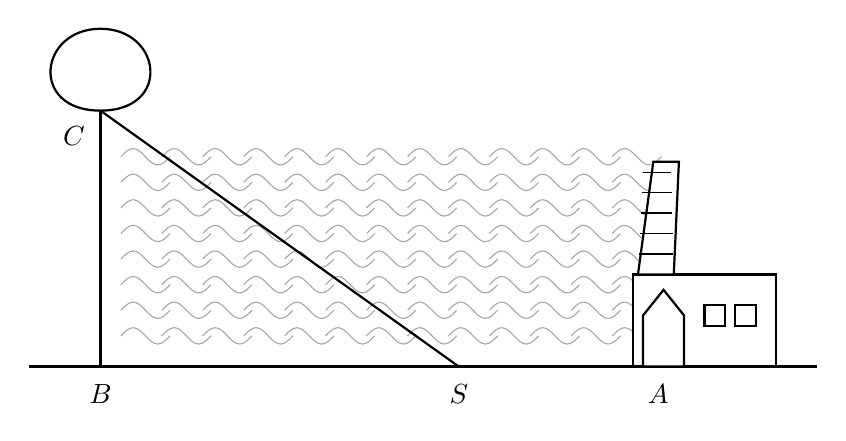
\begin{tikzpicture}[>=stealth, scale=1.3]

    % =================================================================
    % 1. ĐỊNH NGHĨA TỌA ĐỘ CÁC ĐIỂM CHÍNH
    % =================================================================
    \coordinate (B) at (0,0);
    \coordinate (S) at (3.5,0);
    \coordinate (A) at (5.2,0);
    \coordinate (C) at (0,2.5);
    
    % Giới hạn trục nằm ngang mặt đất
    \coordinate (GroundStart) at (-0.7,0);
    \coordinate (GroundEnd) at (7.0,0);

    % =================================================================
    % 2. VẼ NỀN SÓNG NƯỚC (DÒNG SÔNG)
    % =================================================================
    % Điền các ký hiệu sóng nước mờ lặp lại dạng cột để minh họa dòng sông
    \foreach \x in {0.2, 0.6, 1.0, 1.4, 1.8, 2.2, 2.6, 3.0, 3.4, 3.8, 4.2, 4.6, 5.0} {
        \foreach \y in {0.3, 0.55, 0.8, 1.05, 1.3, 1.55, 1.8, 2.05} {
            \draw[shift={(\x,\y)}, xscale=0.6, yscale=0.4, thin, gray!70] 
                (0,0) sin (0.2,0.2) cos (0.4,0) sin (0.6,-0.2) cos (0.8,0);
        }
    }

    % =================================================================
    % 3. VẼ ĐƯỜNG MẶT ĐẤT VÀ CÁC ĐOẠN THẲNG TRONG BÀI TOÁN
    % =================================================================
    % Đường mặt đất nằm ngang
    \draw[thick] (GroundStart) -- (GroundEnd);

    % Đoạn thẳng đứng BC (chiều cao khinh khí cầu) và đường nhìn nghiêng CS
    \draw[thick] (B) -- (C);
    \draw[thick] (C) -- (S);

    % =================================================================
    % 4. VẼ KHINH KHÍ CẦU VÀ NGÔI NHÀ/NHÀ MÁY
    % =================================================================
    % Vẽ khinh khí cầu tại đỉnh C
    \draw[thick, fill=white] (C) .. controls (-0.7, 2.5) and (-0.6, 3.3) .. (0, 3.3)
                             .. controls (0.6, 3.3) and (0.7, 2.5) .. (C) -- cycle;

    % Vẽ ngôi nhà / nhà máy bên phải điểm A
    \begin{scope}[shift={(A)}]
        % Thân nhà chính
        \draw[thick, fill=white] (0,0) rectangle (1.4, 0.9);
        % Cửa ra vào lớn hình vòm nhọn
        \draw[thick, fill=white] (0.1, 0) -- (0.1, 0.5) -- (0.3, 0.75) -- (0.5, 0.5) -- (0.5, 0) -- cycle;
        % Cửa sổ nhỏ vuông bên phải
        \draw[thick] (0.7, 0.4) rectangle (0.9, 0.6);
        \draw[thick] (1.0, 0.4) rectangle (1.2, 0.6);
        % Ống khói cao chia thành từng đốt tầng
        \draw[thick, fill=white] (0.05, 0.9) -- (0.2, 2.0) -- (0.45, 2.0) -- (0.4, 0.9) -- cycle;
        \foreach \h in {1.1, 1.3, 1.5, 1.7, 1.9} {
            \draw[thin] (0.05+\h*0.06-0.06, \h) -- (0.4-\h*0.03+0.03, \h);
        }
    \end{scope}

    % =================================================================
    % 5. GÁN NHÃN ĐỈNH VÀ ĐIỂM
    % =================================================================
    \node[below=3pt] at (B) {$B$};
    \node[below=3pt] at (S) {$S$};
    \node[below=3pt] at (5.45, 0) {$A$};
    \node[below left=3pt] at (C) {$C$};

\end{tikzpicture}
\end{center}

Biết rằng mỗi \( km \) đường ống đặt dưới nước chi phí mất \( 500 \, 000 \, \text{đồng} \), còn đặt dưới đất chi phí mất \( 300 \, 000 \, \text{đồng} \). Chi phí thấp nhất cần bỏ ra để lắp đặt đường ống từ nhà máy \( A \) đến đảo \( C \) là bao nhiêu triệu đồng?}



% --- CÂU 11 ---
\questionShortAnswer{15}{2}{Hai trạm thu phát sóng ở hai vị trí \( A \) và \( B \) nằm về hai phía của một thung lũng. Trạm \( A \) cách thung lũng một khoảng là \( 3 \, \text{km} \), trạm \( B \) cách thung lũng một khoảng là \( 5 \, \text{km} \). Một tuyến cáp quang \( EF \) được thiết kế nối hai điểm đối diện nhau trên bờ thung lũng sao cho \( HE + KF = 15 \, \text{km} \) và độ dài \( EF \) không đổi (được mô hình hóa như hình vẽ bên dưới). Hỏi độ dài \( EH \) là bao nhiêu \( km \) để đường đi từ thành phố \( A \) đến thành phố \( B \) là ngắn nhất (đi theo đường \( AEFB \)) (kết quả làm tròn đến hàng phần trăm)?

\begin{center}
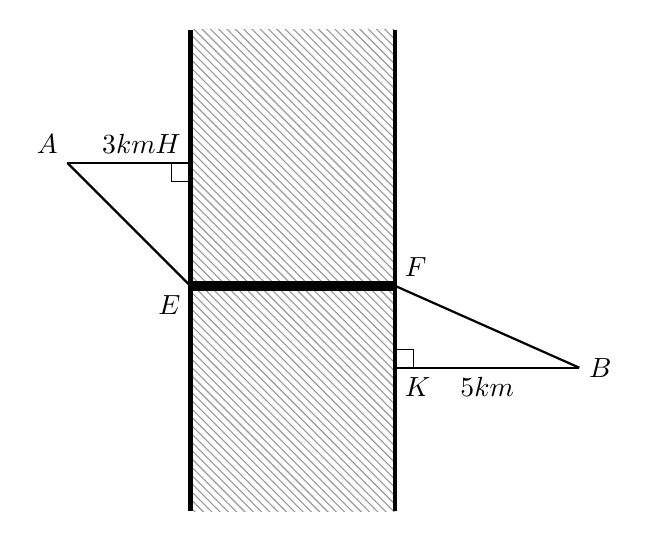
\begin{tikzpicture}[>=stealth, scale=1.3]

    % =================================================================
    % 1. ĐỊNH NGHĨA TỌA ĐỘ CÁC ĐIỂM CHÍNH
    % =================================================================
    \coordinate (H) at (0,1.2);
    \coordinate (E) at (0,0);
    \coordinate (A) at (-1.2,1.2);
    
    \coordinate (F) at (2.0,0);
    \coordinate (K) at (2.0,-0.8);
    \coordinate (B) at (3.8,-0.8);

    % Giới hạn trục dọc hai bờ sông/kênh
    \coordinate (LeftTop) at (0,2.5);
    \coordinate (LeftBottom) at (0,-2.2);
    \coordinate (RightTop) at (2.0,2.5);
    \coordinate (RightBottom) at (2.0,-2.2);

    % =================================================================
    % 2. TÔ VÙNG HỌA TIẾT NỀN GẠCH CHÉO (DÒNG SÔNG) VÀ BIÊN DỌC
    % =================================================================
    % Điền họa tiết gạch chéo xiên làm nền
    \fill[pattern=north west lines, pattern color=gray!80] (LeftBottom) rectangle (RightTop);
    
    % Hai đường biên dọc thể hiện hai bờ sông
    \draw[ultra thick] (LeftBottom) -- (LeftTop);
    \draw[ultra thick] (RightBottom) -- (RightTop);

    % =================================================================
    % 3. VẼ CÁC TUYẾN ĐƯỜNG NỐI VÀ ĐOẠN ĐƯỜNG ĐI LẠI
    % =================================================================
    % Đoạn nằm ngang AH và KB
    \draw[thick] (A) -- (H);
    \draw[thick] (K) -- (B);

    % Đoạn xiên AE và FB
    \draw[thick] (A) -- (E);
    \draw[thick] (F) -- (B);

    % Đoạn cầu nối nằm ngang vuông góc EF (vẽ nét siêu đậm nổi bật trên nền)
    \draw[line width=3.5pt] (E) -- (F);

    % =================================================================
    % 4. VẼ KÝ HIỆU GÓC VUÔNG TẠI H VÀ K
    % =================================================================
    % Góc vuông dưới điểm H
    \draw[thin] (H) ++(0,-0.18) -- ++(-0.18,0) -- ++(0,0.18);
    
    % Góc vuông trên điểm K
    \draw[thin] (K) ++(0,0.18) -- ++(0.18,0) -- ++(0,-0.18);

    % =================================================================
    % 5. GÁN NHÃN ĐỈNH VÀ ĐIỀN THÔNG SỐ KÍCH THƯỚC
    % =================================================================
    % Tên các điểm hình học
    \node[above left] at (A) {$A$};
    \node[above left] at (H) {$H$};
    \node[below left] at (E) {$E$};
    \node[above right] at (F) {$F$};
    \node[below right] at (K) {$K$};
    \node[right] at (B) {$B$};

    % Thông số độ dài khoảng cách
    \node[above] at (-0.6,1.2) {$3km$};
    \node[below] at (2.9,-0.8) {$5km$};

\end{tikzpicture}
\end{center}}




\questionShortAnswer{15}{3}{Một người đưa thư đang ở điểm \( A \), cách điểm \( B \) một đoạn đường xuyên rừng dài \( 60 \, \text{km} \). Trong rừng, người này chỉ có thể di chuyển với vận tốc \( 25 \, \text{km/h} \), và người này cần đến \( B \) trong tối đa \( 2,25 \, \text{giờ} \). May mắn thay, có một con đường nhựa cách đoạn \( AB \) một khoảng \( 12 \, \text{km} \), chạy song song với nó. Trên đường nhựa, người này có thể di chuyển với vận tốc \( 45 \, \text{km/h} \). Biết rằng, nếu di chuyển trên đường nhựa thì người đó sẽ đi theo đường gấp khúc dạng hình thang cân \( ACDB \). Hỏi thời gian ngắn nhất để người đưa thư đi từ \( A \) đến \( B \) là bao nhiêu giờ (kết quả làm tròn đến hàng phần trăm)?

\begin{center}
\begin{tikzpicture}[>=stealth, scale=1.3]

    % =================================================================
    % 1. ĐỊNH NGHĨA TỌA ĐỘ CÁC ĐIỂM CHÍNH
    % =================================================================
    \coordinate (A) at (0,0);
    \coordinate (B) at (6.0,0);
    \coordinate (C) at (1.2,2.5);
    \coordinate (D) at (4.8,2.5);
    
    % Các đỉnh phụ để vẽ đường nét đứt thể hiện chiều cao hình thang
    \coordinate (TopA) at (0,2.5);
    \coordinate (TopB) at (6.0,2.5);
    
    % Giới hạn trục nằm ngang phía dưới
    \coordinate (LineStart) at (-0.7,0);
    \coordinate (LineEnd) at (6.7,0);

    % =================================================================
    % 2. VẼ CÁC ĐƯỜNG THẲNG LIỀN NÉT VÀ NÉT ĐỨT
    % =================================================================
    % Đường nền nằm ngang phía dưới đi qua A và B
    \draw[thick] (LineStart) -- (LineEnd);

    % Đường nhựa nằm ngang phía trên (bao gồm cả các đoạn kéo dài sang hai bên)
    \draw[thick] (TopA) -- (TopB);

    % Hai đường xiên AC và BD
    \draw[thick] (A) -- (C);
    \draw[thick] (B) -- (D);

    % Hai đoạn thẳng đứng thể hiện chiều cao vuông góc (nét đứt)
    \draw[dashed, thick] (A) -- (TopA);
    \draw[dashed, thick] (B) -- (TopB);

    % =================================================================
    % 3. VẼ CÁC ĐIỂM NÚT (CHẤM TRÒN ĐEN)
    % =================================================================
    \fill (A) circle (1.8pt);
    \fill (B) circle (1.8pt);
    \fill (C) circle (1.8pt);
    \fill (D) circle (1.8pt);

    % =================================================================
    % 4. GÁN NHÃN ĐỈNH VÀ ĐIỀN CHÚ THÍCH CHỮ
    % =================================================================
    % Nhãn các điểm hình học
    \node[below left] at (A) {$A$};
    \node[below right] at (B) {$B$};
    \node[above left] at (C) {$C$};
    \node[above right] at (D) {$D$};

    % Thông số khoảng cách/chiều cao 12km
    \node[left=3pt] at (0,1.25) {$12km$};

    % Các nhãn văn bản chú thích địa hình
    \node[above] at (3.0, 2.5) {Đường nhựa};
    \node at (3.0, 1.2) {Rừng};
    \node[below] at (3.0, -0.1) {Rừng};

\end{tikzpicture}
\end{center}}




% --- CÂU 14 ---
\questionShortAnswer{15}{4}{Cho một bờ hồ có dạng nửa đường tròn bán kính bằng 5 km, đường kính \( MN \) như hình vẽ sau:

\begin{center}
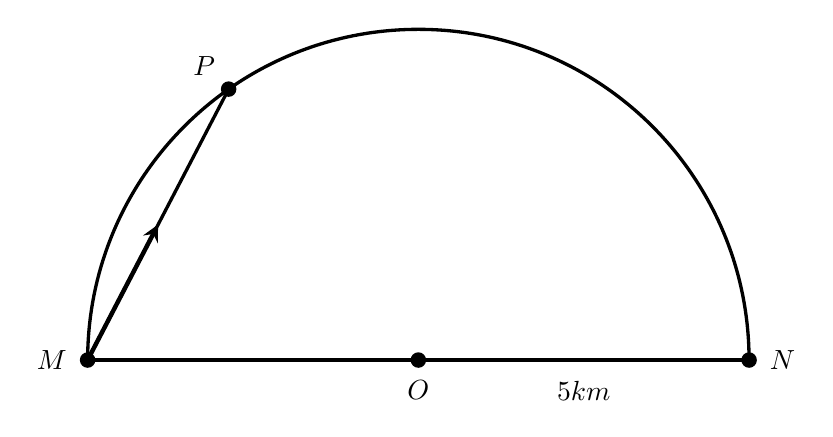
\begin{tikzpicture}[>=stealth, scale=1.4]

    % =================================================================
    % 1. ĐỊNH NGHĨA TỌA ĐỘ VÀ BÁN KÍNH ĐƯỜNG TRÒN
    % =================================================================
    % Tâm đường tròn O đặt tại gốc tọa độ (0,0), bán kính R = 3
    \coordinate (O) at (0,0);
    \coordinate (M) at (-3.0,0);
    \coordinate (N) at (3.0,0);
    
    % Điểm P nằm trên cung tròn (góc khoảng 125 độ tính từ trục Ox)
    \coordinate (P) at ({3.0*cos(125)}, {3.0*sin(125)});

    % =================================================================
    % 2. VẼ ĐƯỜNG KÍNH MN VÀ CUNG TRÒN BÁN NGUYỆT
    % =================================================================
    % Đoạn thẳng đường kính MN liền nét, dày dặn
    \draw[very thick] (M) -- (N);

    % Cung tròn nửa trên từ điểm N quay ngược chiều kim đồng hồ đến M
    \draw[very thick] (3.0,0) arc (0:180:3.0);

    % =================================================================
    % 3. VẼ TIA NỐI MP CÓ CHỨA MŨI TÊN CHỈ HƯỚNG DỊCH CHUYỂN
    % =================================================================
    % Vẽ đoạn thẳng MP
    \draw[very thick] (M) -- (P);
    
    % Vẽ mũi tên chỉ hướng nằm chính giữa đoạn thẳng MP
    \coordinate (MidMP) at ($ (M)!0.5!(P) $);
    \draw[->, ultra thick] (M) -- (MidMP);

    % =================================================================
    % 4. VẼ CÁC ĐIỂM NÚT (CHẤM TRÒN ĐEN)
    % =================================================================
    \fill (M) circle (2.0pt);
    \fill (N) circle (2.0pt);
    \fill (O) circle (2.0pt);
    \fill (P) circle (2.0pt);

    % =================================================================
    % 5. GÁN NHÃN CÁC ĐỈNH VÀ THÔNG SỐ SỐ ĐO
    % =================================================================
    \node[left=4pt] at (M) {$M$};
    \node[right=4pt] at (N) {$N$};
    \node[below=4pt] at (O) {$O$};
    \node[above left=2pt] at (P) {$P$};

    % Điền thông số chiều dài 5km bên dưới đoạn ON
    \node[below] at (1.5,-0.1) {$5km$};

\end{tikzpicture}
\end{center}

Một người Eskimo xuất phát từ điểm \( M \), trượt bằng thuyền kayak trên bảng với vận tốc 5 km/h đến điểm \( P \) trên bờ hồ, rồi chạy bộ trên bảng theo mép hồ đến điểm \( N \) với vận tốc 8 km/h. Hỏi thời gian lớn nhất người Eskimo có thể mất để đi từ \( M \) đến \( N \) là bao nhiêu (thời gian tính bằng giờ, kết quả làm tròn đến hàng phần trăm)?}


% --- CÂU 3 ---
\questionTrueFalse{14}{5}{Hai vận động viên đang ở vị trí A trên bờ cát, cách bờ biển là 5 km. Hai vận động viên cần đến điểm C trên biển để cướp cờ giành chiến thắng. Biết miền ABCD là hình vuông cạnh 10 km. Vận tốc di chuyển trên biển của cả hai vận động viên là 7 km/h và vận tốc di chuyển trên đất liền là 9 km/h. Vận động viên thứ nhất chọn cách di chuyển thẳng từ A đến C. Vận động viên thứ hai chọn cách chạy đến một điểm E nằm trên bờ biển, sau đó bơi về phía C. Đặt \( HE = x \, (km), \, 0 \leq x \leq 10 \).
\begin{center}
    \begin{tikzpicture}[>=stealth, scale=1]

    % =================================================================
    % 1. ĐỊNH NGHĨA TỌA ĐỘ CÁC ĐIỂM CHÍNH (Khung hình chữ nhật 5x4 units)
    % =================================================================
    \coordinate (B) at (0,0);
    \coordinate (A) at (5.0,0);
    \coordinate (D) at (5.0,4.0);
    \coordinate (C) at (0,4.0);
    
    % Các điểm trên trục giữa và đường chéo
    \coordinate (H) at (0,2.0);
    \coordinate (E) at (1.3,2.0);
    \coordinate (EndCoast) at (5.0,2.0);

    % =================================================================
    % 2. VẼ KHUNG HÌNH CHỮ NHẬT VÀ ĐƯỜNG BỜ BIỂN Ở GIỮA
    % =================================================================
    % Khung bao quanh ABCD
    \draw[thick] (B) -- (A) -- (D) -- (C) -- cycle;
    
    % Đường bờ biển nằm ngang ở giữa (H -> EndCoast)
    \draw[thick] (H) -- (EndCoast);

    % =================================================================
    % 3. VẼ CÁC TUYẾN ĐƯỜNG NỐI (C-E-A và C-A)
    % =================================================================
    \draw[thick] (C) -- (E) -- (A);
    \draw[thick] (C) -- (A);

    % =================================================================
    % 4. VẼ GÓC VUÔNG VÀ DẤU NGOẶC ÔM (BRACE) BIỂU DIỄN X
    % =================================================================
    % Ký hiệu góc vuông tại H (nằm góc trên bên phải)
    \draw[thin] (H) ++(0,0.2) -- ++(0.2,0) -- ++(0,-0.2);

    % Dấu ngoặc ôm dưới đoạn HE bằng thư viện hoặc vẽ thủ công mượt mà
    \draw[thin] (0.05, 1.85) .. controls (0.05, 1.75) and (0.6, 1.75) .. (0.65, 1.65)
                .. controls (0.7, 1.75) and (1.25, 1.75) .. (1.25, 1.85);
    \node[below=3pt] at (0.65, 1.65) {$x$};

    % =================================================================
    % 5. GÁN NHÃN CÁC ĐỈNH VÀ THÔNG SỐ ĐỘ DÀI
    % =================================================================
    % Tên các điểm chính
    \node[below left] at (B) {$B$};
    \node[below right] at (A) {$A$};
    \node[above right] at (D) {$D$};
    \node[above left] at (C) {$C$};
    \node[left] at (H) {$H$};
    \node[above right=1pt] at (E) {$E$};

    % Các thông số kích thước hình học
    \node[left] at (0, 3.0) {$5km$};
    \node[left] at (0, 1.0) {$5km$};
    \node[below] at (2.5, 0) {$10km$};

    % Địa danh/Chú thích vùng miền
    \node at (2.8, 3.4) {\textit{biển}};
    \node[above=2pt] at (3.5, 2.0) {\textit{bờ biển}};
    \node at (2.5, 0.3) {\textit{bờ cát}};

\end{tikzpicture}
\end{center}
}{
    \textbf{a)} & Quãng đường di chuyển thẳng từ A đến C của vận động viên thứ nhất là 15 km.
    & \textcolor{amberorange}{$\bigcirc$} & \textcolor{amberorange}{$\bigcirc$} \\ \hline
    
    \textbf{b)} & Tổng thời gian di chuyển của vận động viên thứ hai là  
    \(\dfrac{\sqrt{x^2 + 25}}{10} + \dfrac{10 - x}{7}\) 
    giờ.
    & \textcolor{amberorange}{$\bigcirc$} & \textcolor{amberorange}{$\bigcirc$} \\ \hline
    
    \textbf{c)} & Vận động viên thứ hai đến C ít thời gian nhất khi \( x \approx 3,8 \, km \).
    & \textcolor{amberorange}{$\bigcirc$} & \textcolor{amberorange}{$\bigcirc$} \\ \hline
    
    \textbf{d)} & Vận động viên thứ hai sẽ chiến thắng vận động viên thứ nhất nếu \( HE \approx 3,8 \, km \).
    & \textcolor{amberorange}{$\bigcirc$} & \textcolor{amberorange}{$\bigcirc$} \\
}

% --- CÂU 4 ---
\questionTrueFalse{15}{6}{Bóng đang ở vị trí A cách đoạn đường CD một khoảng 35 km và muốn đến vị trí B cách đoạn đường CD một khoảng 20 km (như hình vẽ). Biết rằng \( CD = 50 \, \text{km} \) và Bóng lái xe theo đường gấp khúc \( AHB \) với vận tốc 40 km/h trên đoạn \( AH \) và 50 km/h trên đoạn \( HB \). Đặt \( HD = x \, (\text{km}) \); \( 0 \leq x \leq 50 \).
\begin{center}
    \begin{tikzpicture}[>=stealth, scale=1.3]

    % =================================================================
    % 1. ĐỊNH NGHĨA TỌA ĐỘ CÁC ĐIỂM CHÍNH
    % =================================================================
    \coordinate (C) at (0,0);
    \coordinate (A) at (0,2.5);
    \coordinate (D) at (5.0,0);
    \coordinate (B) at (5.0,-1.4);
    
    % Điểm giao nhau H (tính toán collinear chính xác)
    \coordinate (H) at (3.2,0);

    % =================================================================
    % 2. VẼ CÁC ĐƯỜNG THẲNG
    % =================================================================
    % Trục ngang CD
    \draw[thick] (C) -- (D);

    % Hai đoạn thẳng đứng AC và BD
    \draw[thick] (A) -- (C);
    \draw[thick] (D) -- (B);

    % Đường chéo xuyên suốt AB đi qua H
    \draw[thick] (A) -- (B);

    % =================================================================
    % 3. GÁN NHÃN CÁC ĐIỂM VÀ GIÁ TRỊ KÍCH THƯỚC
    % =================================================================
    % Tên các đỉnh
    \node[left] at (A) {$A$};
    \node[left] at (C) {$C$};
    \node[right] at (D) {$D$};
    \node[right] at (B) {$B$};
    \node[above right] at (H) {$H$};

    % Các giá trị kích thước
    \node[left] at (0,1.25) {$35$};
    \node[right] at (5.0,-0.7) {$20$};
    
    \node[below] at (1.6, 0) {$50-x$};
    \node[above] at (4.1, 0) {$x$};

\end{tikzpicture}
\end{center}
}{
    \textbf{a)} & Tổng quãng đường Bóng lái xe từ \( A \) đến \( B \) là  
    \(\sqrt{35^2 + (50 - x)^2} + \sqrt{x^2 + 20^2} \, (\text{km}).\)
    & \textcolor{amberorange}{$\bigcirc$} & \textcolor{amberorange}{$\bigcirc$} \\ \hline
    
    \textbf{b)} & Tổng thời gian Bóng lái xe từ \( A \) đến \( B \) là  
    \(50\sqrt{35^2 + (50 - x)^2} + 40\sqrt{x^2 + 20^2} \, (\text{giờ}).\)
    & \textcolor{amberorange}{$\bigcirc$} & \textcolor{amberorange}{$\bigcirc$} \\ \hline
    
    \textbf{c)} & Bóng lái xe ít thời gian nhất khi \( C \) cách \( H \) 15 km (kết quả làm tròn đến hàng đơn vị).
    & \textcolor{amberorange}{$\bigcirc$} & \textcolor{amberorange}{$\bigcirc$} \\ \hline
    
    \textbf{d)} & Thời gian ít nhất để Bóng đến \( B \) là 97 phút (kết quả làm tròn đến hàng đơn vị).
    & \textcolor{amberorange}{$\bigcirc$} & \textcolor{amberorange}{$\bigcirc$} \\
}


\end{document}